\chapter{Turing Machines and Computability}\label{ch:b3:computability}

Some problems have no program at all: not a slow one, not a clever one, none. The school volumes showed one such problem, deciding whether a program halts, with a short argument about programs. This chapter rebuilds that result on a model of computation exact enough to prove things about: the \omterm{def:b3:computability:tm}{Turing machine}. A simulator of thirty lines runs three machines; a second tape changes the speed but not the power; primitive and \omterm{def:b3:computability:recursive}{\(\mu\)-recursive functions} give a second model that computes the same functions; one program runs every machine from its description; and then the limits come, by diagonalisation and by reduction, up to Rice's theorem, which says that no program can decide any \omterm{def:b3:computability:rice}{non-trivial property} of what programs compute. The weekend problem hunts the busy beavers of two states, a function no program computes.

\begin{recall}
The grade-12 chapter on the \omterm{def:b3:computability:halting}{halting problem} showed that no program decides, for every program and input, whether that program halts: from a claimed \omterm{def:b3:computability:languages}{decider} it built a program that does the opposite of what the \omterm{def:b3:computability:languages}{decider} predicts about it. A set is countable when its elements can be listed as a sequence; the set of finite words over a finite alphabet is countable, and Cantor's diagonal argument shows that the set of infinite sequences of bits is not (mathematics volumes). A finite automaton reads its input once, from left to right, and its transition function gives the next state from the current state and the letter read (Year~2 volume).
\end{recall}

\section{More problems than programs}\label{sec:b3:computability:counting}

Before any machine is defined, a count already shows that some problems have no program. A program, in any programming language, is a finite word over a finite alphabet; a problem with yes-or-no answers about natural numbers is a set of natural numbers, the numbers whose answer is yes.

\begin{theorem}[Countably many programs, uncountably many problems]\label{thm:b3:computability:uncountable}
There are countably many programs, and uncountably many sets of natural numbers. Some set of natural numbers is therefore decided by no program.
\end{theorem}

\begin{proof}
List the programs by length, and the programs of each length in alphabetical order: $P_0, P_1, P_2, \ldots$; every program appears at a finite position. Suppose the sets of natural numbers could be listed too, as $A_0, A_1, A_2, \ldots$. The set $D = \{n : n \notin A_n\}$ differs from each $A_n$ on the number $n$, so it is not in the list: a contradiction. If every set were decided by a program, mapping each set to the first program that decides it would list the sets, which is impossible.
\end{proof}

The proof shows that non-computable problems exist but names none. The rest of the chapter makes the argument concrete: it replaces ``set of natural numbers'' by a problem one would like to solve, and ``program'' by a precise machine.

\section{Turing machines}\label{sec:b3:computability:tm}

Alan Turing's paper ``On computable numbers, with an application to the Entscheidungsproblem'', of 1936--37, defined the machine below to say what a person computing with pencil and paper can do. % ledger: b3:turing-1936

\begin{definition}[Turing machine, configuration, transition function of a Turing machine]\label{def:b3:computability:tm}
A \emph{Turing machine}\index{Turing machine} has a finite set of states with a start state, a finite tape alphabet containing a blank symbol, a tape of cells unbounded in both directions, and a head on one cell. Its \emph{transition function}\index{transition function (of a Turing machine)} maps some pairs (state, symbol read) to a triple (new state, symbol written, move left, right or stay). A step applies it; the machine \emph{halts} when no transition applies, and \emph{accepts} if it halts in its accepting state. A \emph{configuration}\index{configuration} is the state, the tape contents and the head position: written $u\,[q]\,v$, the tape left of the head, the state, and the tape from the head on.
\end{definition}

A finite automaton is the special case that only reads and only moves right. Writing, and moving back, is what makes the difference. The simulator stores the tape as a dictionary from positions to symbols, so the tape grows on demand in both directions.

\omcode{code/bachelor-3/15-computability/listings/tm.py}{16}{30}{The simulator's main loop. A machine is a dictionary from (state, symbol) to (state, symbol, move).}\label{lst:b3:computability:tm}

Three machines: a binary increment, which walks to the last digit and carries leftwards; a palindrome checker over $\{a, b\}$, which erases the first letter, remembers it in its state, and checks it against the last; and a unary adder (\code{machines.py}).

\omcode{code/bachelor-3/15-computability/listings/machines.py}{5}{23}{The increment and the palindrome machines as transition tables. \code{B} is the blank.}\label{lst:b3:computability:machines}

\omoutput{code/bachelor-3/15-computability/outputs/machines.txt}{The run of the increment machine on 1011, one \omterm{def:b3:computability:tm}{configuration} per line, then results on other inputs.}\label{out:b3:computability:machines}

\begin{omfigure}
\raisebox{-0.5\height}{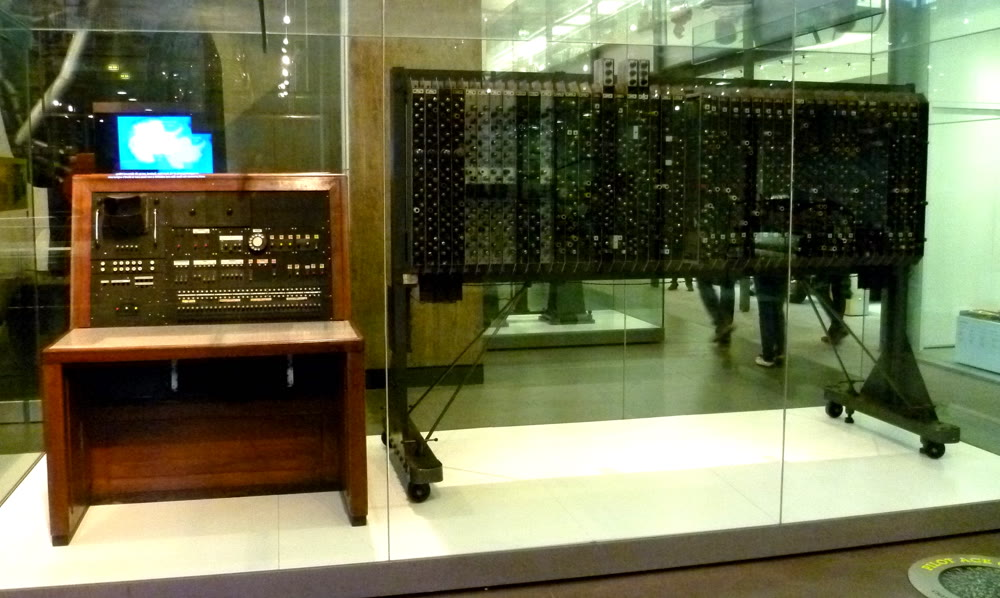
\includegraphics[width=0.44\linewidth]{images/book5/b3-15-pilot-ace.jpg}}\hfill
\begin{tikzpicture}[font=\small, >=Stealth, baseline=(current bounding box.center)]
  \foreach \i/\s in {0/\_, 1/1, 2/0, 3/1, 4/1, 5/\_} {
    \draw (0.7*\i, 0) rectangle ++(0.7, 0.7);
    \node at (0.7*\i + 0.35, 0.35) {\texttt{\s}};
  }
  \node at (-0.3, 0.35) {\dots};
  \node at (4.55, 0.35) {\dots};
  \draw[->, thick] (2.1 + 0.35, -0.75) -- (2.1 + 0.35, -0.05);
  \node[draw, fill=omThm!20, rounded corners] at (2.45, -1.1) {state \texttt{q0}};
  \node[anchor=west] at (0, -1.9) {configuration \texttt{10[q0]11}};
  \node[anchor=west] at (0, -2.4) {next: read 1, write 1, move right};
\end{tikzpicture}
\par\smallskip{\small Left: the Pilot ACE, a cut-down version of Turing's design (Science Museum, London). Right: the increment machine of \cref{out:b3:computability:machines} after two steps.}
\end{omfigure}

The photograph shows the Pilot ACE, one of the first computers built in the United Kingdom, a cut-down version of the design Turing wrote at the National Physical Laboratory; it first ran in 1950. % ledger: b3:pilot-ace
Like every computer since, it is a universal machine in the sense of \cref{sec:b3:computability:universal}: one machine that runs whatever program it is given.

\subsection{More tapes, same power}

A machine with several tapes, one head on each, is easier to program: the palindrome check copies the word to a second tape, then reads the first tape forwards and the second backwards.

\begin{definition}[Multi-tape Turing machine]\label{def:b3:computability:multitape}
A \emph{multi-tape Turing machine}\index{multi-tape Turing machine} with $k$ tapes reads the $k$ symbols under its $k$ heads; its \omterm{def:b3:computability:tm}{transition function} gives the new state, the $k$ symbols written and the $k$ moves. The input starts on the first tape; the others start blank.
\end{definition}

\omcode{code/bachelor-3/15-computability/listings/multitape.py}{23}{34}{The two-tape palindrome machine: copy, rewind the first tape, compare.}\label{lst:b3:computability:multitape}

\omoutput{code/bachelor-3/15-computability/outputs/multitape.txt}{Steps to accept a palindrome of length $n$: about $n^2/2$ with one tape, $3n + 3$ with two.}\label{out:b3:computability:multitape}

The one-tape machine walks the whole word for each pair of letters it crosses off: $(n + 1)(n + 2)/2$ steps. The two-tape machine walks the word three times. The gap is quadratic, and that is the worst that can happen.

\begin{theorem}[One tape simulates $k$]\label{thm:b3:computability:multitape}
For every $k$-tape \omterm{def:b3:computability:tm}{Turing machine} there is a one-tape machine that halts on the same inputs with the same output; if the first takes $t \ge n$ steps on an input of length $n$, the second takes $O(t^2)$ steps.
\end{theorem}

\begin{proof}[Proof idea]
Store the $k$ tapes on one, side by side: cell $i$ of the single tape holds a tuple of $k$ symbols, cell $i$ of each tape, each marked if a head is there (the alphabet of tuples is finite). One step of the $k$-tape machine becomes a sweep: left to right to read the $k$ marked symbols into the state, then back to write and move the marks. After $t$ steps the used part of the tape has at most $n + t \le 2t$ cells, so each sweep costs $O(t)$ steps and the whole run $O(t^2)$.
\end{proof}

Hartmanis and Stearns proved this in 1965, and used multi-tape machines for counting time because they are closer to real computers. % ledger: b3:multitape-hartmanis
A quadratic slowdown changes running times, which \cref{ch:b3:complexity-classes} studies, but it changes nothing about what can be computed at all.

\section{The Church--Turing thesis}\label{sec:b3:computability:thesis}

The \omterm{def:b3:computability:tm}{Turing machine} is one model; the 1930s produced several others, built on quite different ideas. Alonzo Church's 1936 paper used the \(\lambda\)-calculus of \cref{ch:b3:lambda-calculus}. % ledger: b3:church-1936
A third model builds functions on natural numbers from a few basic ones.

\begin{definition}[Primitive recursive function, \(\mu\)-recursive function, Ackermann function]\label{def:b3:computability:recursive}
The \emph{primitive recursive functions}\index{primitive recursive function} are the functions on natural numbers built from zero, the successor $n \mapsto n + 1$ and the projections $(x_1, \ldots, x_k) \mapsto x_i$ by \emph{composition} and by \emph{primitive recursion}: $h(0, \vec y) = g(\vec y)$ and $h(n + 1, \vec y) = s(n, h(n, \vec y), \vec y)$. The \emph{\(\mu\)-recursive functions}\index{mu-recursive function@\(\mu\)-recursive function} also allow \emph{minimisation}: $\mu p(\vec y)$ is the least $n$ with $p(n, \vec y) = 0$, undefined if there is none. The \emph{Ackermann function}\index{Ackermann function} is $A(0, n) = n + 1$, $A(m + 1, 0) = A(m, 1)$, $A(m + 1, n + 1) = A(m, A(m + 1, n))$.
\end{definition}

Primitive recursion is a loop whose number of rounds is known before it starts, a \code{for} loop; minimisation is a \code{while} loop, which may never end. \code{primrec.py} builds both as Python combinators.

\omcode{code/bachelor-3/15-computability/listings/primrec.py}{23}{54}{Primitive recursion, the arithmetic it builds, minimisation and Ackermann's function.}\label{lst:b3:computability:primrec}

\omoutput{code/bachelor-3/15-computability/outputs/primrec.txt}{Addition, multiplication and powers by primitive recursion; a square root by minimisation; Ackermann's function, whose rows grow by $n + 2$, $2n + 3$, $2^{n + 3} - 3$.}\label{out:b3:computability:primrec}

Every \omterm{def:b3:computability:recursive}{primitive recursive function} is total, since every loop ends. Ackermann's function is total too, and computed by the short recursion above, but it is not primitive recursive: each row grows like an iteration of the previous one, and every \omterm{def:b3:computability:recursive}{primitive recursive function} is eventually overtaken by one of the rows. Wilhelm Ackermann gave such a function in 1928, by a nested recursion; the two-argument form above follows Péter's of 1935. % ledger: b3:ackermann-1928
% ledger: b3:ackermann-not-pr
The fourth row already explodes: $A(4, 1) = 65{,}533$, and $A(4, 2) = 2^{65536} - 3$ has 19,729 digits.

\begin{theorem}[The models agree]\label{thm:b3:computability:equivalence}
The total functions computable by a \omterm{def:b3:computability:tm}{Turing machine}, the total \omterm{def:b3:computability:recursive}{\(\mu\)-recursive functions}, the total functions definable in combinatory logic (a relative of the \(\lambda\)-calculus) and the total functions computable by register machines with unbounded registers are the same class; so are the partial functions of the four models.
\end{theorem}

\begin{proof}[Proof idea]
Each model simulates the others. A \omterm{def:b3:computability:tm}{Turing machine} can carry out composition, a bounded loop and an unbounded search on numbers written on its tape. Conversely, a \omterm{def:b3:computability:tm}{configuration} of a \omterm{def:b3:computability:tm}{Turing machine} can be coded as a number, one step is a \omterm{def:b3:computability:recursive}{primitive recursive function} of that code, and minimisation finds the first step at which the machine halts.
\end{proof}

Stephen Kleene gave minimisation its standard form in 1943, and the register machines are Shepherdson and Sturgis's, of 1963. % ledger: b3:kleene-mu
% ledger: b3:models-equivalent

\begin{definition}[Church--Turing thesis]\label{def:b3:computability:thesis}
The \emph{Church--Turing thesis}\index{Church--Turing thesis} states that every function computable by an effective procedure, one that a person could follow mechanically with unlimited paper and time, is computable by a \omterm{def:b3:computability:tm}{Turing machine}.
\end{definition}

The thesis is not a theorem: ``effective procedure'' is not a mathematical notion, so it cannot be proved. It is supported by \cref{thm:b3:computability:equivalence}: every attempt to define computation has given the same class. % ledger: b3:ct-thesis
In practice it lets a proof describe an algorithm in words, or in Python, and conclude that a \omterm{def:b3:computability:tm}{Turing machine} exists.

\section{A universal machine}\label{sec:b3:computability:universal}

A \omterm{def:b3:computability:tm}{Turing machine} is a finite table, so it can be written as a word, and a word can be the input of another machine.

\begin{definition}[Encoding of a machine, universal Turing machine]\label{def:b3:computability:universal}
An \emph{encoding}\index{encoding of a machine} of \omterm{def:b3:computability:tm}{Turing machines} maps each machine $M$ to a word $\langle M \rangle$ over a fixed alphabet, so that the table of $M$ can be computed back from it. A \emph{universal Turing machine}\index{universal Turing machine} $U$ takes $\langle M \rangle$ and a word $w$, and behaves as $M$ on $w$: it halts if and only if $M$ halts, accepts if and only if $M$ accepts, and leaves $M$'s output.
\end{definition}

\code{utm.py} numbers the states, with the start state first, and the symbols, writes each number in unary, and each transition as five numbers separated by 0s; transitions are separated by \texttt{\#}. The universal program decodes the word and runs it.

\omcode{code/bachelor-3/15-computability/listings/utm.py}{10}{30}{\omterm{def:b3:computability:universal}{Encoding} a machine over $\{0, 1, \#\}$, and the universal program that runs an encoded machine.}\label{lst:b3:computability:utm}

\omoutput{code/bachelor-3/15-computability/outputs/utm.txt}{The increment machine as 85 characters, and the same results through the universal program.}\label{out:b3:computability:utm}

A first version numbered the start state 4 instead of 1 and printed its inputs unchanged: \code{named - {start}} had been written inside a union, and \code{-} binds more tightly than \code{|} in Python, so the start state was subtracted from one operand only and listed twice. The test that compares direct and universal runs over every word of length 6 catches that kind of slip. Turing built a universal machine in his 1936--37 paper, as a \omterm{def:b3:computability:tm}{Turing machine}, and used it to prove that some problems have no machine. % ledger: b3:turing-universal
\code{universal} is the same thing in Python; by the thesis, it is a \omterm{def:b3:computability:tm}{Turing machine} too.

\begin{definition}[Decider, decidable language, recognisable language]\label{def:b3:computability:languages}
A machine \emph{recognises} the language of the words it accepts. A language is \emph{recognisable}\index{recognisable language} (semi-decidable, recursively enumerable) when some machine recognises it: on a word of the language it halts and accepts; on another word it rejects or runs for ever. A \emph{decider}\index{decider} is a machine that halts on every input; a language is \emph{decidable}\index{decidable language} when a decider recognises it.
\end{definition}

\begin{theorem}[Decidable means recognisable both ways]\label{thm:b3:computability:complement}
A language $L$ is \omterm{def:b3:computability:languages}{decidable} if and only if $L$ and its complement $\overline{L}$ are both \omterm{def:b3:computability:languages}{recognisable}.
\end{theorem}

\begin{proof}
If a \omterm{def:b3:computability:languages}{decider} $D$ recognises $L$, then $D$ recognises $L$, and $D$ with its answers swapped, still halting on every input, recognises $\overline{L}$. The converse runs the two recognisers side by side; \cref{exo:b3:computability:7} completes it.
\end{proof}

\section{Undecidability}\label{sec:b3:computability:undecidable}

\begin{definition}[Halting problem]\label{def:b3:computability:halting}
The \emph{halting problem}\index{halting problem} is the language $\mathit{HALT} = \{ \langle M, w \rangle : M \text{ halts on } w \}$.
\end{definition}

$\mathit{HALT}$ is \omterm{def:b3:computability:languages}{recognisable}: run the universal machine on $\langle M \rangle$ and $w$, and accept if it halts. It is not \omterm{def:b3:computability:languages}{decidable}. Turing formulated the problem and proved it in the same paper. % ledger: b3:turing-universal

\begin{theorem}[The halting problem is undecidable]\label{thm:b3:computability:halting}
No \omterm{def:b3:computability:tm}{Turing machine} decides $\mathit{HALT}$.
\end{theorem}

\begin{proof}
Suppose a \omterm{def:b3:computability:languages}{decider} $H$ answers whether $M$ halts on $w$. Build the machine $P$ that, on input $\langle M \rangle$, runs $H$ on $\langle M, \langle M \rangle \rangle$, loops for ever if $H$ answers yes, and halts if $H$ answers no. Run $P$ on $\langle P \rangle$. If $P$ halts on $\langle P \rangle$, $H$ answers yes on $\langle P, \langle P \rangle \rangle$, so $P$ loops: a contradiction. If $P$ does not halt, $H$ answers no, so $P$ halts: a contradiction again. So $H$ does not exist.
\end{proof}

The machines $M_0, M_1, \ldots$ against their \omterm{def:b3:computability:universal}{encodings} form a table whose entry $(i, j)$ says whether $M_i$ halts on $\langle M_j \rangle$; $P$ is built to disagree with the diagonal, exactly as the set $D$ of \cref{thm:b3:computability:uncountable} does. \code{diagonal.py} runs the construction against four candidate \omterm{def:b3:computability:languages}{deciders}: each is wrong about the program built from it.

\begin{omfigure}
\begin{tikzpicture}[font=\small]
  \foreach \j in {0,...,4} \node at (1.0*\j + 1.3, 0.5) {$\langle M_\j \rangle$};
  \foreach \i/\r in {0/{H,L,H,H,L}, 1/{L,L,H,L,H}, 2/{H,H,H,L,L}, 3/{L,H,L,L,H}} {
    \node at (0, -0.6*\i) {$M_\i$};
    \foreach \v [count=\j from 0] in \r {
      \ifnum\i=\j \node[draw, fill=omThm!20, minimum size=5mm] at (1.0*\j + 1.3, -0.6*\i) {\v};
      \else \node at (1.0*\j + 1.3, -0.6*\i) {\v};\fi
    }
  }
  \node at (0, -2.55) {$P$};
  \foreach \v [count=\j from 0] in {L,H,L,H} \node[draw, fill=omDef!20, minimum size=5mm] at (1.0*\j + 1.3, -2.55) {\v};
  \node at (5.3, -2.55) {\dots};
  \node[anchor=west, align=left] at (6.2, -1.0) {H: halts, L: loops.\\$P$ flips the diagonal,\\so it differs from every row:\\no row is $P$, yet $P$ is\\a machine if $H$ exists.};
\end{tikzpicture}
\par\smallskip{\small The diagonal argument as a table. The entries are invented for the picture.}
\end{omfigure}

\omcode{code/bachelor-3/15-computability/listings/diagonal.py}{29}{43}{The paradox built from a claimed \omterm{def:b3:computability:languages}{decider}, and four candidate \omterm{def:b3:computability:languages}{deciders}.}\label{lst:b3:computability:diagonal}

\omoutput{code/bachelor-3/15-computability/outputs/diagonal.txt}{Each candidate is wrong on its own paradox: when it says ``halts'' the paradox runs on, when it says ``loops'' the paradox halts.}\label{out:b3:computability:diagonal}

``Is still running'' after 100,000 lines is not a proof that the program never halts; here the program's text shows it, since the branch taken is \texttt{while True:\ pass}. A budget is how every practical tool meets the theorem: it answers ``halts'', ``loops'' for the cases it can prove, and ``don't know'' after its budget.

\subsection{Reductions}

Once one problem is known undecidable, others follow by translating questions.

\begin{definition}[Many-one reduction]\label{def:b3:computability:reduction}
A \emph{many-one reduction}\index{many-one reduction} from a language $A$ to a language $B$ is a computable function $f$ such that $x \in A$ if and only if $f(x) \in B$, for every word $x$. We write $A \le_m B$.
\end{definition}

\begin{theorem}[Reductions transfer undecidability]\label{thm:b3:computability:reduction}
If $A \le_m B$ and $B$ is \omterm{def:b3:computability:languages}{decidable}, then $A$ is \omterm{def:b3:computability:languages}{decidable}. So if $A \le_m B$ and $A$ is undecidable, $B$ is undecidable.
\end{theorem}

\begin{proof}
To decide whether $x \in A$, compute $f(x)$ and run the \omterm{def:b3:computability:languages}{decider} of $B$ on it; both steps halt, and the answer is right because $x \in A \iff f(x) \in B$.
\end{proof}

Take $B = E = \{ \langle N \rangle : N \text{ accepts the empty word} \}$. Given $\langle M, w \rangle$, build $M_w$: it erases its input, writes $w$, returns to its first letter and runs $M$, accepting wherever $M$ halts. Then $M_w$ accepts the empty word, and in fact every word, if and only if $M$ halts on $w$. The map $\langle M, w \rangle \mapsto \langle M_w \rangle$ is computable; \code{reductions.py} computes it.

\begin{omfigure}
\begin{tikzpicture}[font=\small, >=Stealth, box/.style={draw, rounded corners, minimum height=9mm, align=center}]
  \node (in) at (0, 0) {$\langle M, w \rangle$};
  \node[box, fill=omDef!12] (f) at (3.0, 0) {build $M_w$\\(always halts)};
  \node[box, fill=omThm!20] (d) at (7.6, 0) {claimed decider for $E$:\\does $M_w$ accept $\varepsilon$?};
  \node (out) at (11.1, 0) {yes / no};
  \draw[->] (in) -- (f);
  \draw[->] (f) -- node[above, font=\scriptsize] {$\langle M_w \rangle$} (d);
  \draw[->] (d) -- (out);
  \draw[dashed, black!60] (1.3, -0.95) rectangle (9.9, 0.95);
  \node[font=\scriptsize, anchor=north] at (5.6, -0.95) {together: a decider for $\mathit{HALT}$, which cannot exist};
\end{tikzpicture}
\par\smallskip{\small A reduction from $\mathit{HALT}$ to $E$: a \omterm{def:b3:computability:languages}{decider} for $E$ would decide halting.}
\end{omfigure}

\omcode{code/bachelor-3/15-computability/listings/reductions.py}{11}{28}{The reduction $\langle M, w \rangle \mapsto \langle M_w \rangle$, as a transformation of transition tables.}\label{lst:b3:computability:reduction}

\omoutput{code/bachelor-3/15-computability/outputs/reductions.txt}{$M_w$ accepts every word when $M$ halts on $w$, and none when it does not.}\label{out:b3:computability:reduction}

So $E$ is undecidable. So is the emptiness problem, whether $L(N) = \varnothing$: $L(M_w)$ is empty exactly when $M$ does not halt on $w$, and a \omterm{def:b3:computability:languages}{decider} for emptiness, with its answer swapped, would decide halting. And so is equivalence, whether $L(N_1) = L(N_2)$: taking $N_2$ a machine that accepts nothing turns it into emptiness. These are all questions about what a machine accepts; one theorem settles them all.

\begin{definition}[Semantic property, non-trivial property]\label{def:b3:computability:rice}
A property of \omterm{def:b3:computability:tm}{Turing machines} is \emph{semantic}\index{semantic property} when it depends only on the language a machine recognises: two machines with the same language both have it or both lack it. It is \emph{non-trivial}\index{non-trivial property} when some machine has it and some machine lacks it.
\end{definition}

\begin{theorem}[Rice's theorem]\label{thm:b3:computability:rice}\index{Rice's theorem}
Every \omterm{def:b3:computability:rice}{non-trivial} \omterm{def:b3:computability:rice}{semantic property} of \omterm{def:b3:computability:tm}{Turing machines} is undecidable.
\end{theorem}

\begin{proof}
Let $\Pi$ be one. Suppose first that the machines whose language is empty lack $\Pi$, and let $K$ be a machine that has it. Given $\langle M, w \rangle$, build $N$: on input $x$, run $M$ on $w$; if that halts, run $K$ on $x$ and answer as $K$. If $M$ halts on $w$, $L(N) = L(K)$, so $N$ has $\Pi$; if not, $L(N) = \varnothing$, so $N$ lacks $\Pi$. The map $\langle M, w \rangle \mapsto \langle N \rangle$ is computable, so $\mathit{HALT} \le_m \Pi$, and $\Pi$ is undecidable by \cref{thm:b3:computability:reduction}. The other case, where the empty language has $\Pi$, is \cref{exo:b3:computability:10}.
\end{proof}

H. G. Rice published it in 1953. % ledger: b3:rice-1953
It covers ``accepts the empty word'', ``recognises a finite language'', ``recognises a regular language'', ``recognises the same language as this other machine''. It says nothing about properties of the machine's text, such as ``has at most five states'', which is \omterm{def:b3:computability:languages}{decidable}, or ``halts within 1,000 steps on the empty word'', \omterm{def:b3:computability:languages}{decidable} too, by running it.

\begin{definition}[Post correspondence problem]\label{def:b3:computability:pcp}
An instance of the \emph{Post correspondence problem}\index{Post correspondence problem} is a finite list of tiles $(t_1, b_1), \ldots, (t_k, b_k)$, pairs of words; it asks whether some non-empty sequence of indices $i_1, \ldots, i_m$, with repetitions allowed, gives $t_{i_1} \cdots t_{i_m} = b_{i_1} \cdots b_{i_m}$.
\end{definition}

The tiles $(a, baa)$, $(ab, aa)$, $(bba, bb)$ have the match 3, 2, 3, 1: both rows read \texttt{bbaabbbaa}. Emil Post introduced the problem in 1946 and proved it undecidable. % ledger: b3:post-1946
The usual proof builds, from a machine and an input, a set of tiles whose matches spell out the machine's run, so that a match exists if and only if the machine accepts. % ledger: b3:pcp-undecidable
The problem mentions no machine at all, which makes it a convenient starting point for reductions to problems on words and grammars.

\subsection{The busy beaver}

\begin{definition}[Busy beaver function]\label{def:b3:computability:busy-beaver}
Among the \omterm{def:b3:computability:tm}{Turing machines} with $n$ states, a halting state and the symbols 0 and 1, started on a tape of 0s, consider those that halt. The \emph{busy beaver function}\index{busy beaver function} $S(n)$ is the largest number of steps one of them takes, the halting step included; $\Sigma(n)$ is the largest number of 1s one of them leaves.
\end{definition}

Tibor Radó defined it in 1962, as one of the simplest functions no program computes. % ledger: b3:rado-1962
% ledger: b3:bb-definition
For small $n$ a program can still find its values: enumerate every machine and run each one for a while.

\omcode{code/bachelor-3/15-computability/listings/busy_beaver.py}{10}{33}{Every $n$-state machine, run for at most \code{CAP} steps from the blank tape.}\label{lst:b3:computability:busy}

\omoutput{code/bachelor-3/15-computability/outputs/busy_beaver.txt}{All one- and two-state machines: $S(2) = 6$ and $\Sigma(2) = 4$, as the weekend problem confirms.}\label{out:b3:computability:busy}

\begin{theorem}[$S$ is not computable]\label{thm:b3:computability:busy-beaver}
No \omterm{def:b3:computability:tm}{Turing machine} computes $n \mapsto S(n)$.
\end{theorem}

\begin{proof}
If one did, the following would decide whether a two-symbol machine $M$ with $n$ states halts on the blank tape: compute $S(n)$, run $M$ for $S(n)$ steps, and answer ``halts'' if it has halted. A machine that is still running then never halts, since a halting one would have taken at most $S(n)$ steps. But halting on the blank tape is undecidable: the map $\langle M, w \rangle \mapsto \langle M_w \rangle$ of \cref{lst:b3:computability:reduction} reduces $\mathit{HALT}$ to it, once the symbols of $M_w$ are coded in binary, which costs states but not halting.
\end{proof}

\begin{dated}{2026}
Five values of $S$ are known: $S(1) = 1$, $S(2) = 6$, $S(3) = 21$, $S(4) = 107$ and $S(5) = 47{,}176{,}870$, with $\Sigma(5) = 4{,}098$. The fifth was settled by the online bbchallenge collaboration, whose proof, checked by the Coq proof assistant, enumerated 181,385,789 machines; the proof appeared in the spring of 2024 and the paper in 2025. For six states only lower bounds are known, beyond any number that can be written out. % ledger: b3:bb-values
% ledger: b3:bb-2024
\end{dated}

\section{Exercises}\label{sec:b3:computability:exercises}

\begin{exercise}[$\star$]\label{exo:b3:computability:1}
Run the palindrome machine of \cref{lst:b3:computability:machines} on \texttt{aba} for five steps, writing the six \omterm{def:b3:computability:tm}{configurations} from \texttt{[q0]aba}.
\end{exercise}

\begin{exercise}[$\star$]\label{exo:b3:computability:2}
\omterm{def:b3:computability:languages}{Decidable}, \omterm{def:b3:computability:languages}{recognisable} but not \omterm{def:b3:computability:languages}{decidable}, or not even \omterm{def:b3:computability:languages}{recognisable}? (a) The \omterm{def:b3:computability:universal}{encodings} of machines with at most five states. (b) $E$, the machines that accept the empty word. (c) The complement of $E$. (d) The pairs $\langle M, w \rangle$ such that $M$ halts on $w$ within 1,000 steps.
\end{exercise}

\begin{exercise}[$\star$]\label{exo:b3:computability:3}
With the conventions of \code{utm.py}, the symbols of the adder are \texttt{+}, \texttt{1}, \texttt{\_}, numbered 1, 2, 3, and its states \code{q0}, \code{done}, \code{last}. Write the code of the transition $(\mathtt{q0}, \mathtt{+}) \to (\mathtt{q0}, \mathtt{1}, R)$, and that of $(\mathtt{last}, \mathtt{1}) \to (\mathtt{done}, \mathtt{\_}, S)$.
\end{exercise}

\begin{exercise}[$\star$]\label{exo:b3:computability:4}
Predict, without running them: the tape and the number of steps of the increment machine on \texttt{1111}; the tape of the adder on \texttt{1+1}; the number of steps of the palindrome machine on \texttt{aa}.
\end{exercise}

\begin{exercise}[$\star\star$]\label{exo:b3:computability:5}
\code{exercises/ex5_increment.py} gives a binary increment that turns \texttt{111} into \texttt{000}. Find the missing transition and fix it; the test checks every number below 256.
\end{exercise}

\begin{exercise}[$\star\star$]\label{exo:b3:computability:6}
Write a \omterm{def:b3:computability:tm}{Turing machine} for the simulator that accepts exactly the words $a^n b^n$, $n \ge 0$, over $\{a, b\}$. It is tested on every word of length at most 8.
\end{exercise}

\begin{exercise}[$\star\star$]\label{exo:b3:computability:7}
Prove the converse in \cref{thm:b3:computability:complement}: if $L$ and $\overline{L}$ are \omterm{def:b3:computability:languages}{recognisable}, $L$ is \omterm{def:b3:computability:languages}{decidable}. (Run the two recognisers one step each in turn.)
\end{exercise}

\begin{exercise}[$\star\star$]\label{exo:b3:computability:8}
Prove that $\mathit{TOTAL} = \{ \langle M \rangle : M \text{ halts on every input} \}$ is undecidable, by a reduction from $\mathit{HALT}$. Is it a case of Rice's theorem as stated?
\end{exercise}

\begin{exercise}[$\star\star$]\label{exo:b3:computability:9}
Explain the two columns of \cref{out:b3:computability:multitape}: why the two-tape machine takes exactly $3n + 3$ steps on a palindrome of length $n$, and why the one-tape machine takes $(n + 1)(n + 2)/2$.
\end{exercise}

\begin{exercise}[$\star\star\star$]\label{exo:b3:computability:10}
Finish the proof of Rice's theorem: the case where the machines whose language is empty have the property.
\end{exercise}

\begin{exercise}[$\star\star\star$]\label{exo:b3:computability:11}
Let $f$ be any total computable function on natural numbers. Prove that $S(n) > f(n)$ for all large enough $n$. (Build, for each $n$, a machine of $n + c$ states, $c$ fixed, that writes $n$ in unary and then writes a value of $f$ in unary.)
\end{exercise}

\begin{exercise}[$\star\star\star$]\label{exo:b3:computability:12}
With only \code{zero}, \code{succ}, \code{proj}, \code{compose}, \code{primrec} and the functions they already build, define \code{pred} (the predecessor, 0 for 0), \code{monus} ($x \mathbin{\dot-} y$, the difference cut at 0) and \code{div} (integer division for $y > 0$). The test compares them with Python's operators.
\end{exercise}

\section{Weekend problem}\label{sec:b3:computability:problem}

\begin{problem}[{Weekend problem --- The busy beaver}]\label{pb:b3:computability:1}
This problem counts the two-state machines, runs them all, finds the champion of \cref{out:b3:computability:busy} by hand, and proves that no program computes the \omterm{def:b3:computability:busy-beaver}{busy beaver function}. Machines are written as in \code{busy_beaver.py}: \texttt{1LB} means write 1, move left, go to state B; the transitions are listed for A0, A1, B0, B1.

\needspace{4\baselineskip}\medskip\noindent\textbf{Part I --- How many machines.}
\begin{enumerate}
  \item How many actions can one transition take, with $n$ states and a halting state? How many machines with $n$ states are there?
  \item Check the counts 64 and 20,736 of \cref{out:b3:computability:busy}. How many three-state machines are there?
  \item Why do exactly 32 of the 64 one-state machines halt, and why do they all halt after one step?
  \item The five-state proof enumerated 181,385,789 machines. How many five-state machines does the formula of question 1 give? Why can a proof enumerate far fewer?
  \item Two machines that differ only by swapping left and right take the same number of steps. Why?
\end{enumerate}

\needspace{4\baselineskip}\medskip\noindent\textbf{Part II --- Running them all.}
\begin{enumerate}[resume]
  \item Why does \code{busy_beaver.py} need a step cap at all?
  \item What can the cap make the program get wrong, and in which direction?
  \item 9,784 machines halted within 100 steps. Why is it safe to say the other 10,952 never halt, given that $S(2) = 6$ is proved?
  \item Without knowing $S(2)$, what would a cap of 100 prove about $S(2)$?
  \item The test runs every two-state machine for 1,000 steps and finds none that halts after step 6. Why is that evidence, and not a proof?
  \item Give a simple argument proving that a machine never halts when it has no transition to H that can ever be taken from the states it visits.
\end{enumerate}

\needspace{4\baselineskip}\medskip\noindent\textbf{Part III --- The champion.}
\begin{enumerate}[resume]
  \item Run the champion \texttt{1LB 1RB 1RA 1LH} by hand from the blank tape, writing the \omterm{def:b3:computability:tm}{configuration} after each step. How many steps, how many 1s?
  \item Why does its last transition write a 1 rather than a 0?
  \item Write its mirror image. Why does it have the same counts?
  \item The program finds 4 machines that leave four 1s. Which are they?
  \item It finds 40 machines that take six steps. Why many more than for $\Sigma$?
  \item Can a machine take $S(n)$ steps without leaving $\Sigma(n)$ 1s? Use the counts above.
\end{enumerate}

\needspace{4\baselineskip}\medskip\noindent\textbf{Part IV --- No program computes $S$.}
\begin{enumerate}[resume]
  \item Prove $S(n + 1) > S(n)$ for every $n$.
  \item Prove, as in \cref{thm:b3:computability:busy-beaver}, that a program computing $S$ would decide halting on the blank tape.
  \item Why does that contradict \cref{thm:b3:computability:halting}?
  \item From \cref{exo:b3:computability:11}: why does a function that grows faster than every computable function fail to be computable?
  \item Each known value of $S$ needed a proof that every other machine never halts. Why does no single program give those proofs for every $n$?
  \item What does a proof checked by a proof assistant add, for a result that rests on 181 million cases?
  \item Sum up what was computed, and what cannot be.
\end{enumerate}
\end{problem}
